\documentclass{article}
\usepackage[utf8]{inputenc}
\usepackage[margin=0.9in]{geometry}
\usepackage{titling}
\usepackage[utf8]{inputenc}
\usepackage[english]{babel}
\usepackage{amsthm}
\usepackage{amsmath}
\usepackage{amssymb}
\usepackage{graphicx}
\usepackage{changepage}

\graphicspath{ {/home/marko/Problem solving maths group} }
\newtheorem{theorem}{Example}
\newtheorem{exercise}{Exercise}

\title{\textbf{Extreme principle}}
\date{Week 1}
\author{Miroslav Stankovic\\ Marko Puza}
\begin{document}
\maketitle

\section{Theory}

The \emph{Extreme principle}\footnote{https://brilliant.org/wiki/extremal-principle/} is a useful problem solving tactics, or, actually just a very successful and general heuristic. It focuses on \textbf{finding a solution with some extreme property} among all possible candidates (and in the first place, one needs to make sure that such solution actually exists).
In context of number theory, this could mean considering the smallest or largest value, or perhaps the solution with the smallest sum. In context of geometry, it is very often useful to look for the smallest distances, areas or perimeters. In context of graph theory, we could consider the nodes with the smallest/largest degree, the longest path and so on.\\
Afterwards, the solution with the extreme property is used to construct a proof while making use of the simplified conditions that it provides - most often it comes hand in hand with a proof by contradiction.
\\\\
When solving a problem, there can be various hints that somehow suggest that the Extreme principle may be applicable to solve it:
\begin{itemize}
	\item{The set of the possible values is bounded}
	\item{The values in the problem are distinct}
	\item{There is a \emph{monovariant}\footnote{property that only changes in one direction; e.g. non-decreasing property} or \emph{invariant}\footnote{property whose value remains constant} in the problem.}
\end{itemize}


\noindent \\ Having read the above paragraphs, you probably still don't have much of an idea about how the Extreme principle works or why it is of any use. The underlying idea is in fact very simple - and this should become clear by looking at some examples, so let's dive in.

\section{Examples}

\begin{theorem}
There is n sheep standing on a pasture, such that the distances between all pairs of them are \textbf{distinct}. Each one of them is peacefully chewing grass waiting for the shepherd dog to bark. Once the dog barks, every sheep will start staring at the nearest sheep. Show that after the bark, there is a pair of sheep awkwardly staring at each other.
\end{theorem}

\begin{proof}
Consider the smallest distance between two sheep (there must be such, since there is only finitely many sheep). For these two, the nearest sheep to them is necessarily the other one and thus they will choose to stare at each other.
\end{proof}

%\begin{theorem}
%Prove that there is infinitely many primes.
%\end{theorem}

%\begin{proof}
%By contradiction. Suppose there is only a finite number of primes. \\ Let $p_{1}, p_{2}, p_{3}, ..., p_{n}$ be all primes in increasing order and define number $N$ as: \\
%$N = p_{1} \cdot p_{2} \cdots p_{n} + 1$ \\
%Notice, that $N$ is coprime to every $p_{i}$.
%Now, either $N$ is prime itself, in which case it must be larger than $p_{n}$, or there exists a prime factor of $N$ that is not among $p_{1}, p_{2}, ..., p_{n}$ and thus is also larger than $p_{n}$. This contradicts the fact that $p_{n}$ is largest prime. \qedhere
%\\\\
%In this example, we made use of the largest prime (Extreme principle!).
%\end{proof}

\break

\begin{theorem}
Show that there is no quadruple $x, y, z, u$ of natural numbers satisfying
$x^{2} + y^{2} = 3(z^{2} + u^{2})$.
\end{theorem}

\begin{proof}
By contradiction. Suppose there exists at least one solution for the given equation. From all solutions $(x, y, z, u)$, take the one for which sum $x + y + z + u$ is the smallest (we know that such solution must exist, since the set of natural numbers is lower-bounded). \\\\
Notice now, that $x^{2} + y^{2} \equiv 0 \pmod 3$. Since a square can only have remainders $0, 1$ when divided by $3$, the only case where this equation can hold is $x^{2} \equiv y^{2} \equiv 0 \pmod 3$ (convince yourself). Hence $x = 3k$ and $y = 3l$ for some natural numbers $k, l$. \\
Therefore:
\begin{align*}
{(3k)}^{2} + {(3l)}^{2} &= 3(z^{2} + u^{2})\\
9k^{2} + 9l^{2} &= 3(z^{2} + u^{2}) \\
3(k^{2} + l^{2}) &= z^{2} + u^{2}
\end{align*}
At this point, we can see that quadruple $(z, u, k, l)$ is also a valid solution. Furthermore, $z + u + k + l < z + u + 3k + 3l = z + u + x + y$, which contradicts our assumption that $(x, y, z, u)$ was the solution with the smallest sum. \qedhere
\\\\
Here, we conveniently used the minimal property of some solution (Extreme principle!).
\end{proof}

\begin{theorem}
There are $n$ points given on a plane. \textbf{Each} three of them determine a triangle whose area is at most $1$. Show that all points lie inside a triangle whose area is at most $4$.
\end{theorem}

\begin{proof}
From among all triples of points, let $(A, B, C)$ be the triple that determines triangle with the largest area. Now consider line $l_{A}$ parallel to $BC$. Notice that there are no points behind this line (denoted area in the picture).
If there was any point $P$ in there, its distance from $BC$ would be greater than distance of $A$ from $BC$, which would result in the area of triangle $PBC$ greater than the area of $ABC$. That would yield a contradiction.
\begin{center}
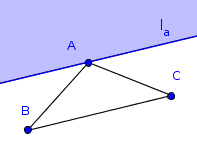
\includegraphics[width=0.3\textwidth]{img1}
\end{center}
Now define lines $l_{B}, l_{C}$ in a same manner and denote $K = l_{B} \cap l_{C},\\ L = l_{A} \cap l_{C}$ and $M = l_{A} \cap l_{B}$. By the same arguments, we know that all points must lie inside the interior of triangle $KLM$.
\begin{center}
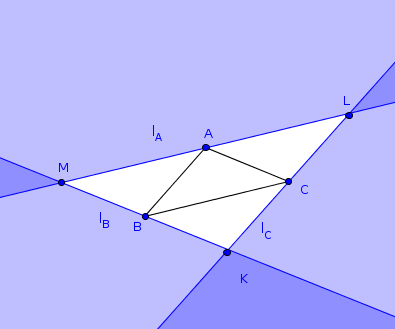
\includegraphics[width=0.45\textwidth]{img2}
\end{center}
Finally, just notice that segments $AB, BC, AC$ are mid-segments of a triangle $KLM$ and they divide it into $4$ congruent parts. Area of $ABC$ is at most one and thus area of $KLM$ is at most $4$, which is exactly what we wanted to prove.
\end{proof}

\begin{exercise}
Have you ever encountered a proof using extreme properties? What were they? Try to think of as many extreme properties that could be usable for the Extreme principle as possible.
\end{exercise}

\begin{exercise}
Try to think of some cases where the solutions with extreme properties \emph{don't} exist. Roughly, what are the conditions for extreme properties to exist?
\end{exercise}

\section{Problems}

\begin{enumerate}

%new for year 2
	\item{There are $n$ points on a plane. No line passes through exactly two of those points. Prove that all $n$ points lie on a line.}

	\item{Using extreme principle prove that every tree has at least two vertices with degree 1.}

	\item{We're given a pentagon. Is it always possible to choose three of its sides and construct a triangle? What if we use diagonals?}

	\item{Prove that every convex polyhedron has at least two faces with the same number of sides.}

	\item{Is there a tetrahedron such that each of it's edges forms an obtuse angle (with some other edge)?}
%end of new

	\item{Consider an infinite chessboard, the squares of which have been filled with \textbf{positive} integers. Each of these integers is the arithmetic mean of four of its neighbors [above, below, left, right]. Show that all the integers are equal to each other.}

	\item{$2n$ points are chosen in the plane such that no $3$ are collinear. $n$ are coloured blue and $n$ are coloured red. Prove that there is a way to join the $n$ red points to the $n$ blue points by $n$ line segments, such that no two line segments cross.}

%	\item{For $n>1$, the integers from 1 to $n^2$ are placed in the cells of an $n\times n$ chessboard. Show that there is a pair of horizontally, vertically, or diagonally adjacent cells whose value differs by at least $n+1$}

%	\item{Fifteen sheets of paper of various sizes and shapes lie on a desktop covering it completely. The sheets may overlap and may even hang over the edge. Show that five of the sheets may be removed so that the remaining ten sheets cover at least $2/3$ of the desktop.}

	\item{There are $n>1$ points in the plane, not all collinear. Prove that there exists a line passing through exactly $2$ points.}

	\item{(a) Let $p(x)$ be a polynomial such that for all $x$, $p(x) + p'(x) \ge 0$. Does it follow that for all $x$, $p(x) \ge 0$?
\\(b) Suppose $p(x)$ is a smooth function, but not necessarily a polynomial. Does the answer to (a) change?}

%	\item{Prove that a cube cannot be divided (\emph{cubed}) into finite number of \textbf{distinct} smaller cubes. What about \emph{hypercubing} a hypercube? \\
%(\textsc{hint\footnote{it is \textbf{possible} to \emph{square} a square.})}}

%	\item{Let $m, n$ be possitive integers and $a_1, a_2, ..., a_n$ be distinct elements of $\{1, 2, ..., n\}$ such that whenever $a_i + a_j \le n$ for some $i, j$ with $1\le i\le j\le m$, there exists $k$, $1 \le k \le m$, with $a_i + a_j = a_k$. Prove that
%	\[\dfrac{a_1 + a_2 + ... + a_m}{m} \ge \dfrac{n+1}{2}\]}

	\item{In the coordinate plane, prove that the vertices of a regular pentagon cannot all have integer coordinates.}

	\item{What is the maximum number of regions defined by $n$ lines in a plane?}

    \item{All plane sections of a solid are circles. Prove that the solid is a sphere.}

    \item{$2015$ vectors are drawn on a plane. Two players alternately take a vector until there are no more vectors left. The winner is the player whose vectors’ sum is longer. Suggest a winning (or at least a non-losing) strategy for the first player}.

    \item{Suppose there are $n$ lines on a plane such that every two lines intersect and through any intersection point of two lines there goes at least one other line. Prove that all lines intersect in one point.}

\end{enumerate}
\end{document}

Bonus:
All plane sections of a solid are circles. Prove that the solid is a ball.

Bonus 2:
$2015$ vectors are drawn on a plane. Two players alternately take a vector until there are no more vectors left. The winner is the player whose vectors’ sum is longer. Suggest a winning (or at least a non-losing) strategy for the first player.

Sources:
https://web.viu.ca/bigelow2/Math360ClassProblemsInvolvingExtremePrinciple.pdf
https://www.math.hmc.edu/~ajb/PCMI/pcmi10_b.pdf
https://brilliant.org/wiki/extremal-principle/
http://www.artofproblemsolving.com/wiki/index.php/Extreme_principle
https://www.math.wisc.edu/wiki/images/Putnam112013.pdf
